%%%%%%%%%%%%%%%%%%%%%%%%%%%%%%%%%%%%%%%
% Resume/CV
% LaTeX Template
% Version 1.1 (23,10,2022)
%
% Original author:
% Saurabh Chorge
%https://github.com/MrSaurabh75
%%%%%%%%%%%%%%%%%%%%%%%%%%%%%%%%%%%%%%


%----------------------------------------------------------------------------------------
%	PACKAGES AND OTHER DOCUMENT CONFIGURATIONS
%----------------------------------------------------------------------------------------


\documentclass[letterpaper,10pt]{memoir} % Font and paper size
\usepackage{hyperref}
\usepackage{fontawesome}





%%%%%%%%%%%%%%%%%%%%%%%%%%%%%%%%%%%%%%%%%
% Resume/CV
% LaTeX Template
% Version 1.1 (23,10,2022)
%
% Original author:
% Saurabh Chorge
%https://github.com/MrSaurabh75
%%%%%%%%%%%%%%%%%%%%%%%%%%%%%%%%%%%%%%%%%

%----------------------------------------------------------------------------------------
%	PACKAGES AND OTHER DOCUMENT CONFIGURATIONS
%----------------------------------------------------------------------------------------

\usepackage{XCharter} % Use the Bitstream Charter font
\usepackage[utf8]{inputenc} % Required for inputting international characters
\usepackage[T1]{fontenc} % Output font encoding for international characters

\usepackage[top=1cm,left=1cm,right=1cm,bottom=1cm]{geometry} % Modify margins

\usepackage{graphicx} % Required for figures

\usepackage{flowfram} % Required for the multi-column layout

\usepackage{url} % URLs

\usepackage[usenames,dvipsnames]{xcolor} % Required for custom colours

\usepackage{tikz} % Required for the horizontal rule

\usepackage{enumitem} % Required for modifying lists
\setlist{noitemsep,nolistsep} % Remove spacing within and around lists

\setlength{\columnsep}{\baselineskip} % Set the spacing between columns

% Define the left frame (sidebar)
\newflowframe{0.2\textwidth}{\textheight}{0pt}{0pt}[left]
\newlength{\LeftMainSep}
\setlength{\LeftMainSep}{0.2\textwidth}
\addtolength{\LeftMainSep}{1\columnsep}
 
% Small static frame for the vertical line
\newstaticframe{1.5pt}{\textheight}{\LeftMainSep}{0pt}
 
% Content of the static frame with the vertical line
\begin{staticcontents}{1}
\hfill
\tikz{\draw[loosely dotted,color=RoyalBlue,line width=1.5pt,yshift=0](0,0) -- (0,\textheight);}
\hfill\mbox{}
\end{staticcontents}
 
% Define the right frame (main body)
\addtolength{\LeftMainSep}{1.5pt}
\addtolength{\LeftMainSep}{1\columnsep}
\newflowframe{0.7\textwidth}{\textheight}{\LeftMainSep}{0pt}[main01]

\pagestyle{empty} % Disable all page numbering

\setlength{\parindent}{0pt} % Stop paragraph indentation

%----------------------------------------------------------------------------------------
%	NEW COMMANDS
%----------------------------------------------------------------------------------------

\newcommand{\userinformation}[1]{\renewcommand{\userinformation}{#1}} % Define a new command for the CV user's information that goes into the left column

\newcommand{\cvheading}[1]{{\Huge\bfseries\color{RoyalBlue} #1} \par\vspace{.6\baselineskip}} % New command for the CV heading
\newcommand{\cvsubheading}[1]{{\Large\bfseries #1} \bigbreak} % New command for the CV subheading

\newcommand{\Sep}{\vspace{1em}} % New command for the spacing between headings
\newcommand{\SmallSep}{\vspace{0.5em}} % New command for the spacing within headings

\newcommand{\aboutme}[2]{ % New command for the about me section
\textbf{\color{RoyalBlue} #1}~~#2\par\Sep
}
	
\newcommand{\CVSection}[1]{ % New command for the headings within sections
{\Large\textbf{#1}}\par
\SmallSep % Used for spacing
}

\newcommand{\CVItem}[2]{ % New command for the item descriptions
\textbf{\color{RoyalBlue} #1}\par
#2
\SmallSep % Used for spacing
}

\newcommand{\bluebullet}{\textcolor{RoyalBlue}{$\circ$}~~} % New command for the blue bullets
 % Include the file specifying document layout and packages

%----------------------------------------------------------------------------------------
%	NAME AND CONTACT INFORMATION 
%\usepackage{pgf}

\userinformation{ % Set the content that goes into the sidebar of each page

\begin{flushleft}
    

% Comment out this figure block if you don't want a photo
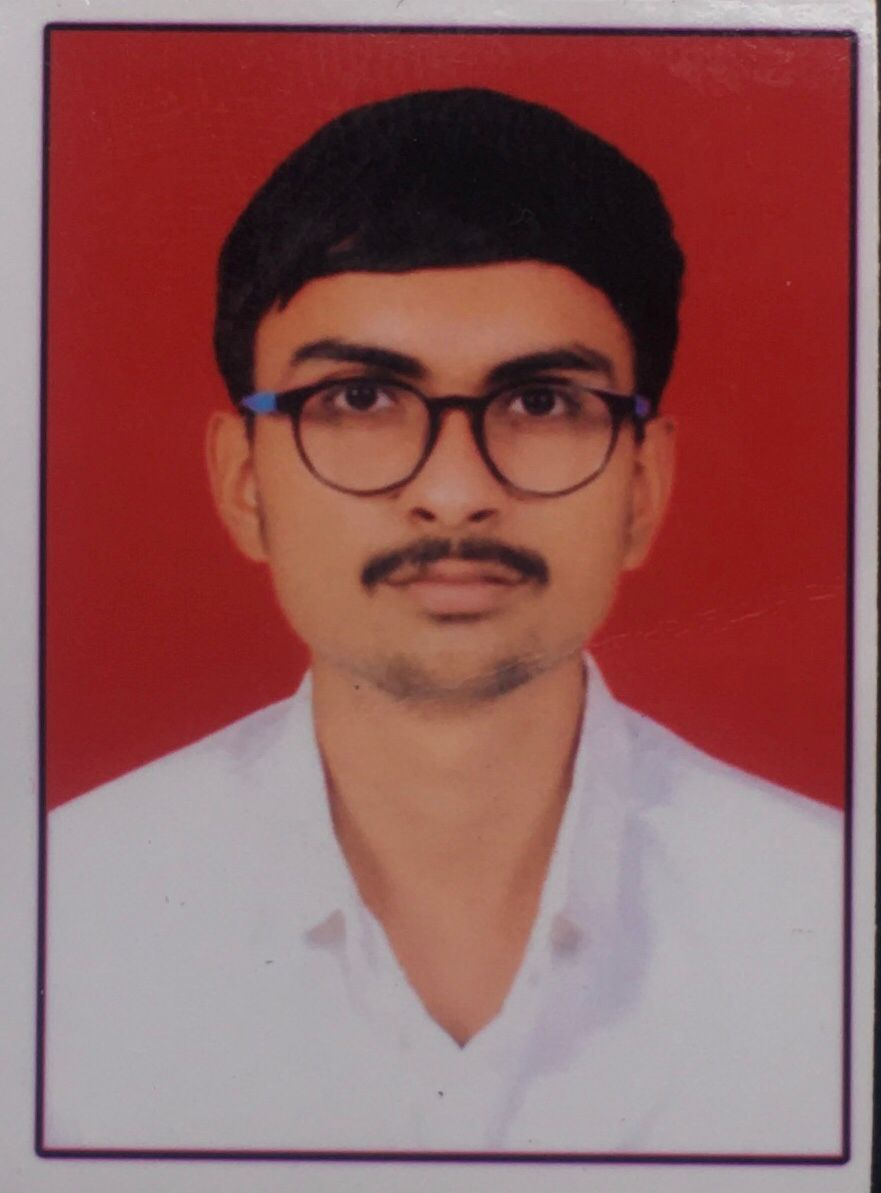
\includegraphics[width=0.7\columnwidth]{saurabhchorge.jpeg}\\[\baselineskip] % Your photo
\small % Smaller font size
\textbf{Saurabh Digambar Chorge}\\[\baselineskip]  % Your name
\textbf{\faEnvelope \hspace{.1cm} E-mail :} \\
\href{mailto:saurabhdc7575@gmail.com}{saurabhdc7575 @gmail.com} \\ % Your email address
[\baselineskip] 
\textbf{\faPhone \hspace{.1cm} Phone :}\\
\href{tel:9130701209}{+91 9130701209}\\[\baselineskip]

\textbf{\faBirthdayCake \hspace{.1cm} Date of Birth :}\\
{March 13, 2002}\\[\baselineskip]

\textbf{\faMale \hspace{.1cm} Gender :}\\
\hspace{0.4cm}{Male}\\[\baselineskip]

\textbf{\faLink \hspace{.1cm} Marital Status :}\\
\hspace{.4cm}{Unmarried}\\

\Sep % Some whitespace
\textbf{\faMapMarker \hspace{.1cm} Address :} \\
Dattanagar , Chinchwad ,\\ % Address 1
Pune , Maharashtra,\\ % Address 2
India , 411033\\[\baselineskip]% Address 3



\textbf{\faLanguage \hspace{.1cm} LANGUAGES}\Sep
%------------------------------------------------
\begin{itemize} 

    \item Marathi : Native Tongue
    \item Hindi
    \item English

\end{itemize}
\\[\baselineskip]
\textbf{\faAngellist \hspace{.1cm} HOBBIES}\Sep
\begin{itemize} 

    \item Sports : Cricket
    \item Reading
    \item Watching Movies
    \item Gaming
    
\end{itemize}
\Sep\Sep
\textbf{\href{https://www.linkedin.com/in/saurabh-chorge-237996202/}{\faLinkedinSquare \hspace{.1cm} Linkedin}}\\[\baselineskip]

\textbf{\href{https://github.com/MrSaurabh75}{\faGithubSquare \hspace{.1cm} GitHub}}\\[\baselineskip]

\vfill % Whitespace under this block to push it up under the photo
\end{flushleft}
}




%----------------------------------------------------------------------------------------

\begin{document}
\userinformation % Print your information in the left column

\framebreak % End of the first column

%----------------------------------------------------------------------------------------
%	HEADING
%----------------------------------------------------------------------------------------

\cvheading{Saurabh Digambar Chorge } % Large heading - your name

\cvsubheading{\faLaptop \hspace{.1cm} M.C.A - Master Of Computer Application} % Subheading - your occupation/specialization

%----------------------------------------------------------------------------------------
%	Objective
%----------------------------------------------------------------------------------------

\aboutme{Objective}

{Seeking to leverage academic and practical acumen gathered in clinching opportunities in reputed company for both personal and professional growth.}\\

%----------------------------------------------------------------------------------------
%	EDUCATION
%----------------------------------------------------------------------------------------

\CVSection{\faGraduationCap \hspace{.1cm} EDUCATION}

%------------------------------------------------

\CVItem{Bachelor of Science (B.Sc), Computer Science}

{2019 - 2022}\\
{Prof. Ramkrushna More College, Pune}\\
{Savitribai Phule Pune University}\\
CGPA : 7.77/10\\
\textbf{\href{https://drive.google.com/file/d/1Y_d1f7XW1VYKLRC9zUc6Hj5_W-hmOaE0/view?usp=sharing}{Certificate}}\\



%------------------------------------------------

\CVItem{Senior Secondary (XII), Science}

{Year of completion: 2019}\\
{Abasaheb Chinchwade Jr. College, Akurdi}\\
{MAHARASHTRA STATE board}\\
Percentage: 62.77\% \\
\textbf{\href{https://drive.google.com/drive/u/0/folders/10_GHjB540w3rGgFYKoydtyAJAjgOLdYw}{Certificate}}\\

\CVItem{Secondary (X)}

{Year of completion: 2017}\\
{New English School, Chinchwad}\\
{MAHARASHTRA STATE board}\\
Percentage: 79.60\% \\
\textbf{\href{https://drive.google.com/drive/u/0/folders/10_GHjB540w3rGgFYKoydtyAJAjgOLdYw}{Certificate}}\\

\CVSection{\faBriefcase \hspace{.1cm} INTERNSHIPS}
%------------------------------------------------

\CVItem{Vitrual Intern}

{Accenture, Pune}\\
{Dec 2022 - Jan 2023}\\
\textbf{\href{https://drive.google.com/drive/u/0/folders/10_GHjB540w3rGgFYKoydtyAJAjgOLdYw}{Completion Certificate}}
\begin{itemize}
	\item Define technical requirements, Design changes to an existing architecture, Scale on-premise systeminfrastructure to the cloud, Reading and understanding code, Attention to detail.

	\item Debugging algorithms, Unit testing, User Acceptance Testing - UAT, Security maturity assessment, IAM policies and permissions.

	\item Securing the software development lifecycle (SDLC), Shaping the Problem, Data and privacy.\\
\end{itemize}\\


%----------------------------------------------------------------------------------------
\CVSection{\faSimplybuilt \hspace{.1cm} PROJECTS}

\CVItem{Amazon Clone Web Application}

{Feb 2022 - Mar 2022}\\
\begin{itemize}
    \item t is a web based application which serves two purposes 1 The system will be used for general purpose like customer's can see the products and can add the products into the cart and can checkout the final amount. 2 For the frontend React JS is used and for the backend purpose Firebase is used, and it’s deployed live hosted online on firebase .\\
\end{itemize}
%----------------------------------------------------------------------------------------
\clearpage % Start a new page

\framebreak
\framebreak

%----------------------------------------------------------------------------------------
\Sep

\CVItem{Quiz Game}

{Nov 2023 - Dec 2023}\\
{GitHub Link : \href{https://github.com/MrSaurabh75/BrainQuiz}{https://github.com/MrSaurabh75/BrainQuiz}}
\begin{itemize}
    \item Developed and launched "BrainQuiz" app, seamlessly blending entertainment and education through a personalized 10-question quiz experience with a 15-second time limit per question, inclusive of a 50:50 lifeline for strategic engagement. Designed a user-friendly interface, fostering active participation and providing instant feedback to enhance knowledge expansion in a dynamic digital learning environment.\\
\end{itemize}

\CVItem{Personal Portfolio}

{Dec 2023 - Jan 2024}\\
{GitHub Link : \href{https://github.com/MrSaurabh75/Portfolio}{https://github.com/MrSaurabh75/Portfolio}}
\begin{itemize}
    \item Crafted a dynamic personal portfolio showcasing my skills, projects, and achievements. Designed an intuitive user interface for easy navigation, offering a comprehensive overview of my professional journey and highlighting key accomplishments in various fields. The portfolio serves as a compelling digital representation of my skills and expertise..\\
\end{itemize}

\CVItem{E-Commerce Website}

{Jan 2024}\\
{GitHub Link : \href{https://github.com/MrSaurabh75/AMSportWebSite}{https://github.com/MrSaurabh75/AMSportWebSite}}
\begin{itemize}
    \item Developed a dynamic e-commerce website for a sports shop using HTML, CSS, and JavaScript. Implemented a user-friendly interface with seamless navigation, showcasing a diverse range of sports products. The incorporation of responsive design ensures an optimal viewing experience across various devices, enhancing the overall shopping experience.\\
\end{itemize}
%------------------------------------------------

\Sep % Extra whitespace after the end of a major section

\CVSection{\faFlask \hspace{.1cm} TECHNICAL SKILLS}

\CVItem{Java \hspace{4cm} Python}{Intermediate \hspace{4.6cm} Intermediate}\\

\CVItem{Data Structures \hspace{4cm} DBMS}{Intermediate \hspace{4.6cm} Beginner}\\

\CVItem{HTML \hspace{5.6cm} CSS}{Intermediate \hspace{4.6cm} Intermediate}\\

\CVItem{JavaScript}{Beginner}\\
%----------------------------------------------------------------------------------------
\CVSection{\faWpforms \hspace{.1cm} CERTIFICATIONS}

\CVItem{Python 3.7 Udemy}{\href{https://drive.google.com/file/d/1DHyhOo37_snAvFe4xsdvQq2uDsWLvhbG/view}{Certificate}}\\

\CVItem{Python For Data Science & Machine Learning}{\href{https://drive.google.com/file/d/1Rq-HvafFxlq-AqnHOuy3csA594vNkJVh/view}{Certificate}}\\

\CVItem{JavaScript}{\href{https://drive.google.com/file/d/18yZRODw0Z0sKXLvFmEo7CCERufUp3afL/view}{Certificate}}\\

%\CVItem{Python Kaggle \hspace{4.2cm} C++ Udemy}{\href{https://drive.google.com/file/d/1T8nd8zAvOjSjYAAmB9n-R4lp_Dmvb6qQ/view?usp=sharing}{Certificate} \hspace{5cm} \href{https://drive.google.com/file/d/19mJye2IQ5M-D3EjD2Wydg6oGMwQL2WDo/view?usp=sharing}{Certificate}}\\%

%----------------------------------------------------------------------------------------

\Sep % Extra white space after the end of a major section
\end{document}
